\documentclass[a4paper, 11pt] {article}
\usepackage[margin=2cm]{geometry}
\usepackage{placeins}
\usepackage{Float}
\usepackage{graphicx}
\usepackage{wrapfig}
\graphicspath{{/.}}
\begin{document}
\title{ECM2414 Card Game Coursework}
\author{690037391 \& 680039372}
\date{\today}
\maketitle
	\begin{center}
		Marks Split: 50:50
	\end{center}
\pagebreak
\section*{Development Log}
\begin{center}
\begin{table}[H]
\begin{tabular}{|l|l|l|l|l|}
\hline
Date           & Time     & Duration  & Roles                                                 & Signature                       \\ \hline
 26/10/2020 & 11:30    & 1hr 40m  & Driver: 680039372, Navigator: 690037391 & 680039372 \& 690037391 \\ \hline
 26/10/2020 & 13:20    & 1hr 40m  & Driver: 690037391, Navigator: 680039372 & 680039372 \& 690037391 \\ \hline
 26/10/2020 & 15:00    & 2hr 00m & Driver: 680039372, Navigator: 690037391 & 680039372 \& 690037391 \\ \hline
 27/10/2020 & 11:30    & 2hr 00m & Driver: 690037391, Navigator: 680039372 & 680039372 \& 690037391 \\ \hline
 27/10/2020 & 13:30 & 2hr 00m & Driver: 680039372, Navigator: 690037391 & 680039372 \& 690037391 \\ \hline
 28/10/2020 & 11:30 & 1hr 30m & Driver: 690037391, Navigator: 680039372 & 680039372 \& 690037391 \\ \hline
 28/10/2020 & 13:00 & 3hr 00m & Driver: 680039372, Navigator: 690037391 & 680039372 \& 690037391 \\ \hline
 05/11/2020 & 13:10 & 2hr 50m & Driver: 690037391, Navigator: 680039372 & 680039372 \& 690037391 \\ \hline
\end{tabular}
\end{table}
\end{center}
\FloatBarrier
\pagebreak
\section*{Production Code Design}
\subsection*{Preliminary User Input}
The \texttt{CardGame} class will query the user for the initial parameters to setup the game, such as the number of players and the path to the file specifying the cards in the game. Once the system is provided with the correct information, the next phase will start.
\subsubsection*{Number of Player Query}
If the user doesn't enter a valid input (a positive integer), the system should explain that the input is invalid and it should ask the user for the correct input.
\subsubsection*{Pack File Query}
If the user doesn't enter a real path, the system should explain and ask the user to input a real path.
Should a real file be provided, the system should check each line to see if it is a positive integer, and if not, it should explain to the user that the file they provided contains invalid cards. It should then ask the user to provide another path to a valid deck.

Should all the cards in the file be valid, the system then check to see if the amount of cards found is equal to $8n$, $n$ being the number of players in the game. If it has too many or too little cards, the system should explain that to the user and ask for a new file that has the right amount of cards.
\subsection*{Player Class}
The \texttt{Player} class implements the \texttt{Runnable} interface and represents a player as a thread. 
The \texttt{Player} should have a public \texttt{playerNumber} (the number assigned to a player) and a private \texttt{hand} (which is a list of \texttt{Card} instances). 
The \texttt{Player} will have 1 getter method, \texttt{getNumberOfCards()} which returns the number of cards. 
It will also have two action methods, \texttt{addToHand(Card card)} and \texttt{discardCard(Card card)}. The former will add the card to the hand or throw a \texttt{HandFullException} if the hand is full (contains 4 cards). The latter will remove the card from the hand or throw a \texttt{HandEmptyException} if the hand is empty. 
The predicate \texttt{hasWon()} returns a boolean depending on whether a player's hand meets the winning condition. 
The \texttt{takeTurn(CardDeck deckLeft, CardDeck deckRight)} method combines both actions into a single atomic action, wherein a player takes a card from the left, checks if it is preferred and either adds it to their hand if it is or discards the card to their right if it does not. 
Finally, this class overrides the \texttt{Runnable run()} method, implementing a locking system between threads (seen in the \textbf{Locking} subsection).

\subsection*{CardDeck Class}
The \texttt{CardDeck} class has a private final \texttt{deckNumber} (the number assigned to the deck) and an \texttt{ArrayDeque<Card> deck)} which is a Double ended queue of \texttt{Card} objects, allowing for insertion of a card at the end of the queue and taking of a card from the head of the queue. This class also has a getter method (\texttt{getDeckNumber()}) which returns the number of the deck. This class also has an \texttt{addCard(Card card)} and a \texttt{removeCard(Card card)} method which adds a card to the \texttt{deck} queue or remove a card from the \texttt{deck} queue respectively. Finally, this class has a \texttt{takeCard()} method which returns and removes the head of the \texttt{deck} queue, allowing for a player to take a card from the top of a deck.

\subsection*{Card Class}
The \texttt{Card} class represents the cards themselves and has a single \texttt{final int denomination} attribute which represents the integer denomination and has a constructor which sets the \texttt{denomination}.

\subsection*{CardGameUtil Class}
This class holds methods that can be abstracted outside of the CardGame itself to allow for more general use, especially for testing. It contains the necessary methods for creating and clearing text files and for adding and removing lines. It also contains the synchronized method for notifying a thread's lock. This is one of the most important methods in this game as, without it, the threads would remain in a deadlock.

\subsection*{CardGame Class}
This class holds the functionality for the game itself and also contains the \texttt{main} method for this project. The CardGame has a few atomic booleans which identify whether a player has won or whether a thread should shutdown and rejoin the main game thread. It also contains lists of cards, players and threads. When a card game is created, it initializes the various lists needed. Card game contains a method \texttt{setupInput} which is responsible for retrieving the user's input from the command line or via an input stream if passed as an argument. 
A pack is loaded via a \texttt{BufferedReader and FileReader}, which reads in the text file and does the necessary checks on them (i.e. are there 8\textit{n} cards?). Then, \texttt{setupGame()} sets up the necessary player and deck objects, and adds them to the respective lists. It then continues to distribute cards between Players and then Decks in a round-robin fashion. 
The next methods are responsible for the threads themselves, namely \texttt{setupThreads(), waitForShutdown()} and \texttt{shutdown()}. The setupThreads method creates a new thread for each player and starts them. The waitForShutdown method waits for all threads to finish executing current actions and then joins them into the main thread. Finally, shutdown method sets the shutdown flag to true, hence invoking waitForShutdown.
Finally, we have multiple getter methods for the various lists and class attributes.

\subsection*{Locking System}
\begin{wrapfigure}{r}{0.3\textwidth}
\centering
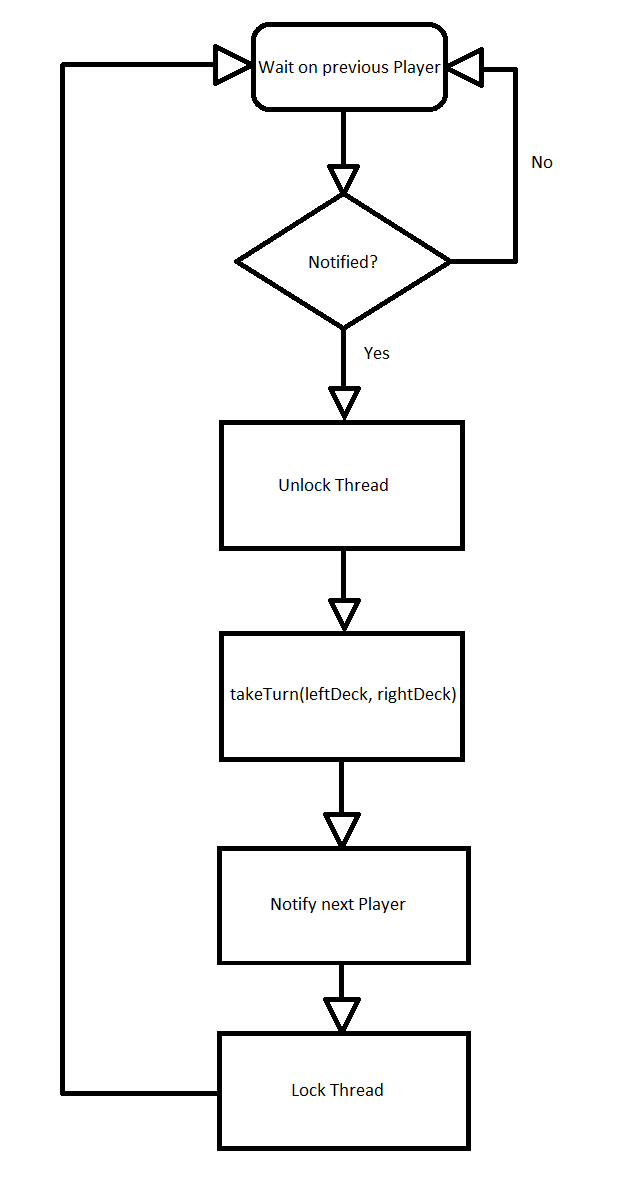
\includegraphics[width=0.3\textwidth]{thread_locking.png}
\end{wrapfigure}

To prevent deadlocking and other concurrency issues, a simple locking system will be put into place. In this system, all \texttt{Player} threads are created, run and then all set to wait on a lock on the previous player in the ring system (i.e. Player 1 waits on Player 4, Player 3 waits on Player 2). The main program thread in which the \texttt{CardGame} main method runs will notify the first Player, who removes their lock and which invokes their \texttt{takeTurn} method; once a player finishes their turn, they proceed to notify the next player in the ring and then lock themselves. This creates a loop around the ring of waiting, unlocking, taking turns, notifying the next player, locking and waiting for the previous player. This loop will only end when a Shutdown flag is sent to all players, making them join into the main thread (effectively terminating them). See to the right a flowchart of the locking system.


\pagebreak
\section*{Testing Design}
\subsection*{Framework}
We will be using JUnit 4 for all of our unit tests and for our testing suite, alongside Eclipse IDE. Overall, we have 6 test classes. Below, we will go through each test class, highlighting the more important tests from within those.

\subsection*{CardDeckTest}
Firstly, \texttt{testCardDeck()} tests that the CardDeck constructor instantiates a CardDeck object correctly. It does this by retrieving the deckNumber via Java Reflections and setting that it has been set to the correct value. If any of the Exceptions that can be thrown by the \texttt{getDeclaredField} method are thrown, the test fails. If the set \texttt{deckNumber} does not equal the intended deck number, the test fails. This test was created to ensure a CardDeck can be created with the correct attributes, including those that are set through arguments. Tests also exist for adding cards to and removing cards from a deck (using new Card objects) alongside a test for taking a card from the deck; testing the addition and removal of cards to a deck is vital to the running of the game. This covers all functionalities of the CardDeck itself; alongside this we also test that, when taking a card, an exception is thrown if the deck is empty to prevent the case of a player picking up a Card that does not exist.

\subsection*{CardTest}
This test class has a single test within it that tests the constructor of the Card object. It checks that the set denomination is equal to the intended denomination, failing if they are not equal. This test was created to ensure a Card can be instantiated correctly with the intended denomination.

\subsection*{PlayerTest}
We have a test for the constructor, checking that a player is instantiated correctly. There is also a test that serves a dual purpose as the method of testing is exactly the same. To test the addition of a card to a player's hand, one must get their hand and to test that you can get a players hand, one must add cards to it. Thus, we have decided to test both in one test, having multiple assertions for the failure cases of both adding to and getting a hand.
Tests for boolean predicates such as \texttt{isPreferred} (is a denomination preferred?) and \texttt{hasWon} (has a player won with their current hand?) work by checking the card denomination and putting a player in a win-condition, respectively.
A test for a player taking their turn sets a player up with a full hand, creates two decks (one to the left, one to the right) and creates a new \texttt{CardGame}. The player then takes their turn, with failure cases occurring if a hand is empty, a hand is full or if a deck is empty. The results of this test is outputted to a directory (\texttt{/cardsTest/Tests}) independent from the regular outputs (\texttt{/cardsTest/Output}).

Finally, a test for deadlocking tests that a player does not deadlock in a game of 2 players with a set input (namely \texttt{/cardsTest/Tests/validTestPack.txt}). This does this by using Java Reflection to retrieve a list of the currently active threads for the game and then checking that, after 5 seconds, the threads do not enter the \texttt{WAITING} state at the same time. The performance cost of this test is very large compared to others, with it taking at least 5 seconds to complete; however, we feel that it is a necessary amount of time to ensure that deadlocking does not exist in the selected amount of time (comparable to how long a larger game could take).

\subsection*{CardGameUtilTest}
This test class is responsible for all testing of the reading and writing to files. We have tests for writing to a file that create a new empty text file and then write a single line to it, asserting that the contents and length of the file are as intended (1 line of the intended content). Testing the clearing of a file requires asserting that a file of length \textit{n} now has a length of 0.

Finally, this test class is also responsible for testing the \texttt{notifyLock()} method, which notifies the next player in turn to lock. It does this by creating an \texttt{Object lock} and setting it to wait. When the new thread is started, if the thread takes longer than 3 seconds to start waiting, the test reaches it's timeout and fails. Then, the thread's lock is notified and should progress the thread to \texttt{RUNNABLE} and then to \texttt{TERMINATED}. Again, if this takes longer than 3 seconds it will time out and the test will fail. This test works over timeouts to ensure that a thread executes in an acceptable amount of time and also changs between different states via the lock in a reasonable amount of time.

\subsection*{CardInputTest}
This class is responsible for testing multiple different edge cases for what a user could input during the selection of number of players and the card pack itself. It does this by creating a \texttt{ByteArrayInputStream} and feeding a string containing selections in. There are multiple cases, but some include: 2 Player Valid Pack, 2 Player with non-integer Pack, 2 Player with invalid pack sizes and a 1 Player game with a valid input pack. These tests have all been designed around 2 players as larger pack sizes take longer to check through.

\subsection*{CardGameTest}
Finally, this class is responsible for testing that the game itself runs. It does this by, firstly, testing that a cardgame can be instantiated correctly in the constructor method. If any of the required players, decks, cards or threads fail to be instantiated, the test will fail.
The next test will check that the Shutdown flag is sent correctly and that all threads join back into the main thread correctly; if any thread fails to join, the test will fail. 

Finally, the \texttt{testSetupGame()} tests that a game is set up, players and decks are initialised and that cards are successfully distributed amongst them. To do this, we set up an Input Stream that will contain the input needed to start a 4 player game with a pack tailored to allow a win from the players. If the number of players is not 4, the number of decks is not 4 or cards are not distributed correctly between hands and decks then the test will fail.

\end{document}